
在LLVM中,值是有独特的构造——不仅表示存储在变量中的值,还模拟了从常量、全局变量、单个指令,甚至基本块等广泛的概念。换句话说,它是LLVM IR的基础。

值的概念对于指令特别重要,因为它直接与IR中的值交互。因此,在本节将对它们进行相同的讨论。我们将了解值在LLVM IR中是如何工作的,以及值是如何与指令相关联的。在此之上,我们将了解如何创建和插入新的指令,以及如何更新它们。

为了学习如何在LLVM IR中使用值,我们必须理解这个系统背后的重要理论,它规定了LLVM指令的行为和格式——单一静态赋值(SSA)形式。

\subsubsubsection{10.3.1\hspace{0.2cm}SSA}

\textbf{SSA}是一种构造和设计IR的方法,可以使程序分析和编译器转换更容易执行。在SSA中,一个变量(在IR中)只会赋值一次。这意味着不能像这样操作一个变量:

\begin{lstlisting}[style=styleCXX]
// the following code is NOT in SSA form
x = 94;
x = 87; // `x` is assigned the second time, not SSA!
\end{lstlisting}

尽管一个变量只能被赋值一次,但它可以在任意指令中多次使用:

\begin{lstlisting}[style=styleCXX]
x = 94;
y = x + 4; // first time `x` is used
z = x + 2; // second time `x` is used
\end{lstlisting}

读者们可能想知道普通的C/C++代码(显然不是SSA形式)如何转换成SSA形式的IR,比如:LLVM。虽然有很多不同的算法和研究论文可以回答这个问题,但我们不打算在这里讨论,大多数简单的C/C++代码都可以通过一些简单的技术进行转换,比如:重命名。例如,假设我们有以下(非SSA)C代码:

\begin{lstlisting}[style=styleCXX]
x = 94;
x = x * y; // `x` is assigned more than once, not SSA!
x = x + 5;
\end{lstlisting}

这里,我们可以在第一个赋值语句中重命名\texttt{x},在第二个和第三个赋值语句的左边分别使用\texttt{x0}和\texttt{x}这样的名称,例如:\texttt{x1}和\texttt{x2}:

\begin{lstlisting}[style=styleCXX]
x0 = 94;
x1 = x0 * y;
x2 = x1 + 5;
\end{lstlisting}

通过这些简单的技巧,我们可以获得具有相同行为的原始代码的SSA。

为了对SSA有一个更全面的理解,必须改变我们对程序中指令的思考方式。在\textbf{命令式编程语言}(如C/C++)中,经常将每个语句(指令)视为一个\textbf{动作},例如:在下面的图中,在左边,第一行表示“将94赋给变量x”的操作,第二行表示“在将结果存储到变量x之前,使用x和y做一些乘法”:

\hspace*{\fill} \\ %插入空行
\begin{center}
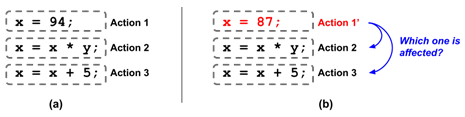
\includegraphics[width=0.8\textwidth]{content/3/chapter10/images/4.png}\\
图10.4 - 将指令视为“动作”
\end{center}

这些解释听起来很直观。然而,当我们对这些指令进行一些转换时(当然,这是编译器中常见的事情),事情就变得棘手了。在图中,在右边,当第一条指令变成\texttt{x = 87}时,我们不知道这个修改是否会\textbf{影响}其他指令。如果会影响,我们还不确定哪一个指令会受到影响。这个信息不仅告诉我们是否有其他潜在的优化机会,而且它也是编译器转换正确性的关键因素——毕竟,没有人希望在启用优化时编译器会破坏原始的代码。更糟糕的是,假设我们要检查\textbf{动作3}右边的\texttt{x}变量。我们感兴趣的是修改这个\texttt{x}的最后几条指令。在这里,我们只能列出所有左边有\texttt{x}的指令(也就是说,使\texttt{x}作为目标),这非常的低效。

我们可以把注意力集中在指令所产生的数据上,从而清楚地了解每条指令的来源——也就是结果值可以到达的区域。此外,我们可以很容易地找到任意变量/值的原点。下图说明了这样做的优势:

\hspace*{\fill} \\ %插入空行
\begin{center}
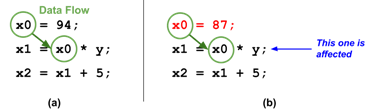
\includegraphics[width=0.7\textwidth]{content/3/chapter10/images/5.png}\\
图10.5 - SSA显示指令之间的数据流
\end{center}

换句话说,SSA显示程序中的\textbf{数据流},以便编译器更容易地跟踪、分析和修改指令。

LLVM中的指令以SSA形式组织。这意味着我们更感兴趣的是由指令生成的值或数据流,而不是将结果存储在哪个变量中。因为LLVM IR中的每条指令只能产生一个结果值,\texttt{Instruction}对象——\texttt{Instruction}是在LLVM IR中表示一条指令的C++类——也可以表示它的\textbf{结果值}。更具体地说,LLVM IR中值的概念是由一个C++类\texttt{Value}表示的。\texttt{Instruction}是它的子类。这意味着给定一个\texttt{Instruction}对象,当然,我们可以将它强制转换为一个\texttt{Value}对象。这个特定的\texttt{Value}对象实际上是该\texttt{Instruction}的结果:

\begin{lstlisting}[style=styleCXX]
// let's say `I` represents an instruction `x = a + b`
Instruction *I = …;
Value *V = I; // `V` effectively represents the value `x`
\end{lstlisting}

这是使用LLVM IR最重要的事情之一,特别是在使用它API时。

虽然\texttt{Instruction}对象表示它自己的结果值,但也有作为指令输入的操作数。你猜怎么着?我们也使用\texttt{Value}对象作为操作数。例如,有以下代码:

\begin{lstlisting}[style=styleCXX]
Instruction *BinI = BinaryOperator::Create(Instruction::Add,…);
Instruction *RetI = ReturnInst::Create(…, BinI, …);
\end{lstlisting}

前面的代码片段基本上创建了一个算术加法指令(由\texttt{BinaryOperator}表示),它的结果值将是另一个返回指令的操作数。生成的IR等价于下面的C/C++代码:

\begin{lstlisting}[style=styleCXX]
x = a + b;
return x;
\end{lstlisting}

除了\texttt{Instruction}之外,\texttt{Constant}(C++中用于不同类型常量的类)、\texttt{GlobalVariable}(C++中用于全局变量的类)和\texttt{BasicBlock}都是\texttt{Value}的子类。这意味着它们也是以SSA的形式组织的,并且可以将它们用作指令的操作数。

现在,了解了SSA是什么,并了解了它对LLVM IR设计的影响。下一节中,我们将讨论如何修改和更新LLVM IR中的值。

\subsubsubsection{10.3.2\hspace{0.2cm}值}

SSA使我们关注指令之间的数据流。由于我们对值如何从一条指令传递到另一条指令有了清晰的认识,因此很容易在指令中替换某些值的使用。但“值”的概念在LLVM中是如何体现的呢?下面的图表显示了两个回答这个问题的重要C++类——\texttt{User}和\texttt{Use}:

\hspace*{\fill} \\ %插入空行
\begin{center}
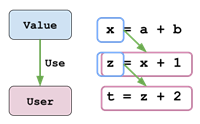
\includegraphics[width=0.5\textwidth]{content/3/chapter10/images/6.png}\\
图10.6 - Value、User和Use之间的关系
\end{center}

\texttt{User}代表了一个IR实例(例如,一条指令)的概念,它使用了一个特定的\texttt{Value}。此外,LLVM还使用了另一个类\texttt{Use}来创建\texttt{Value}和\texttt{User}之间的边界。\texttt{Instruction}是\texttt{Value}的子类——\texttt{Value}表示由该\texttt{Instruction}生成的结果。事实上,\texttt{Instruction}也是从\texttt{User}派生出来的,因为所有的\texttt{Instruction}都至少有一个操作数。

多个\texttt{Use}实例可能指向一个\texttt{User},这意味着\texttt{User}使用了多个\texttt{Value}实例。可以使用\texttt{User}提供的\texttt{value\_op\_iterator}来检索每个\texttt{Value}实例,例如:

\begin{lstlisting}[style=styleCXX]
// `Usr` has the type of `User*`
for (Value *V : Usr->operand_values()) {
	// Working with `V`
}
\end{lstlisting}

同样,\texttt{operand\_values}只是一个实用函数,用于生成\texttt{value\_op\_iterator}的范围。

下面是我们为什么要遍历\texttt{Value}的所有\texttt{User}实例的一个例子:假设我们正在分析一个程序,其中一个\texttt{Function}实例将返回敏感信息——比如,一个\texttt{get\_password}函数。我们的目标是确保每当在函数中调用\texttt{get\_password}时,返回值(敏感信息)不会通过另一个函数调用而遭到泄露。例如,我们想要检测以下的模式,并发出警报:

\begin{lstlisting}[style=styleCXX]
void vulnerable() {
	v = get_password();
	…
	bar(v); // WARNING: sensitive information leak to `bar`!
}
\end{lstlisting}

实现此分析的最常用的原生方法是,检查敏感\texttt{Value}的所有\texttt{User}实例。下面是示例代码:

\begin{lstlisting}[style=styleCXX]
User *find_leakage(CallInst *GetPWDCall) {
	for (auto *Usr : GetPWDCall->users()) {
		if (isa<CallInst>(Usr)) {
			return Usr;
		}
	}
…
}
\end{lstlisting}

\texttt{find\_leaks}函数接受一个\texttt{CallInst}参数——表示调用\texttt{get\_password}函数——并返回任何使用该\texttt{get\_password}调用返回的\texttt{Value}实例的\texttt{User}实例。

一个\texttt{Value}实例可以被多个不同的\texttt{User}实例使用。类似地,我们可以使用下面的片段来遍历它们:

\begin{lstlisting}[style=styleCXX]
// `V` has the type of `Value*`
for (User *Usr : V->users()) {
	// Working with `Usr`
}
\end{lstlisting}

至此,我们了解了如何检查\texttt{Value}的\texttt{User}实例,或者当\texttt{User}使用的\texttt{Value}实例。此外,当我们开发编译器转换时,将\texttt{User}使用的\texttt{Value}实例更改为另一个实例是很常见的操作。LLVM提供了一些方便的工具来完成这项工作。

首先,\texttt{Value::replaceAllUsesWith}方法可以,正如它的名字所示的那样,告诉它的所有\texttt{User}实例使用另一个\texttt{Value}来代替原始的。下图说明了它的效果:

\hspace*{\fill} \\ %插入空行
\begin{center}
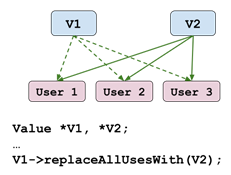
\includegraphics[width=0.5\textwidth]{content/3/chapter10/images/7.png}\\
图10.7 - Value::replaceAllUsesWith的效果
\end{center}

当用另一个\texttt{Instruction}替换相应\texttt{Instruction}时,这个方法非常有用。使用前面的图表来解释这一点,\texttt{V1}是原来的\texttt{Instruction},\texttt{V2}是新\texttt{Instruction}。

另一个实现类似功能的函数是\texttt{User::replaceUsesOfWith(From,To)}。此方法有效地扫描\texttt{User}中的所有操作数,并将特定\texttt{Value}(From参数)的使用替换为另一个\texttt{Value}(To参数)。

在本节中学习的技能是在LLVM中开发程序转换的一些基本工具。下一节中,我们将讨论如何创建和修改指令。

\subsubsubsection{10.3.3\hspace{0.2cm}指令}

之前,我们了解了\texttt{Value}的基础知识——包括与指令的关系——以及在SSA框架下更新\texttt{Value}实例的方法。本节中,我们将了解一些更基本的知识和技能,可以更好地理解指令,并以正确和有效的方式修改指令实例,这是开发一个成功编译器优化的关键。

下面是我们将在本节讨论的内容:

\begin{itemize}
\item 不同指令类型之间的强制转换
\item 插入新指令
\item 更换指令
\item 批量处理指令
\end{itemize}

让我们从不同的指令类型开始。

\hspace*{\fill} \\ %插入空行
\noindent
\textbf{不同指令类型之间的强制转换}

前一节中,我们了解了一个名为\texttt{InstVisitor}的程序,\texttt{InstVisitor}类可以确定指令实例的底层类。它还省去了在不同指令类型之间进行强制转换的工作。然而,我们不能总是依赖\texttt{InstVisitor}来处理每一个涉及到指令,及其派生类之间类型转换的任务。更简单地说,我们想要一个父类和子类之间类型转换的简单解决方案。

C++已经通过\texttt{dynamic\_cast}指令提供了这种机制,对吗?下面是一个\texttt{dynamic\_cast}的例子:

\begin{lstlisting}[style=styleCXX]
class Parent {…};
class Child1 : public Parent {…};
class Child2 : public Parent {…};

void foo() {
	Parent *P = new Child1();
	Child1 *C = dynamic_cast<Child1*>(P); // OK
	Child2 *O = dynamic_cast<Child2*>(P); // Error: bails out at
	// runtime
}
\end{lstlisting}

在代码中使用的\texttt{foo}函数中,可以在它的第二行中看到,可以将\texttt{P}转换为一个\texttt{Child1}实例,因为这是它的底层类型。另一方面,我们不能将\texttt{P}转换成\texttt{Child2}——如果这样做,程序会在运行时崩溃。

实际上,\texttt{dynamic\_cast}具有我们正在寻找的确切功能——更正式地说,是\textbf{运行时类型信息(RTTI)}特性——但它在运行时性能方面也有很高的开销。糟糕的是,C++中RTTI的默认实现相当复杂,使得生成的程序难以优化。因此,LLVM默认关闭RTTI功能。由于这个原因,LLVM提出了自己的运行时类型转换系统,这个系统更加简单和高效。本节中,我们将讨论如何使用它。

LLVM的类型转换框架为动态类型转换提供了三个功能:

\begin{itemize}
\ttfamily
\item isa<T>(val)
\item cast<T>(val)
\item dyn\_cast<T>(val)
\end{itemize}

第一个函数\texttt{isa<T>}——发音为"is-a"——检查\texttt{val}指针类型是否可以转换为\texttt{T}类型的指针。下面是一个例子:

\begin{lstlisting}[style=styleCXX]
// `I` has the type of `Instruction*`
if (isa<BinaryOperator>(I)) {
	// `I` can be casted to `BinaryOperator*`
}
\end{lstlisting}

注意,与\texttt{dynamic\_cast}不同,在这种情况下,不需要将\texttt{BinaryOperator*}作为模板参数——只需要一个没有指针限定符的类型。

\texttt{cast<T>}函数执行从(指针类型)\texttt{val}到\texttt{T}类型指针的实类型转换。下面是一个例子:

\begin{lstlisting}[style=styleCXX]
// `I` has the type of `Instruction*`
if (isa<BinaryOperator>(I)) {
	BinaryOperator *BinOp = cast<BinaryOperator>(I);
}
\end{lstlisting}

同样,不需要将\texttt{BinaryOperator*}作为模板参数。注意,如果在调用\texttt{cast<T>}前没有使用\texttt{isa<T>}执行类型检查,程序将在运行时崩溃。

最后一个函数\texttt{dyn\_cast<T>},是\texttt{isa<T>}和\texttt{cast<T>}的组合。如果适用,可以执行类型转换。否则,返回null。下面是一个例子:

\begin{lstlisting}[style=styleCXX]
// `I` has the type of `Instruction*`
if (BinaryOperator *BinOp = dyn_cast<BinaryOperator>(I)) {
	// Work with `BinOp`
}
\end{lstlisting}

这里,我们可以看到一些简洁的语法,将变量声明(\texttt{BinOp})与\texttt{if}语句结合在一起。

注意,这些API都不能以null作为参数。相反,\texttt{dyn\_cast\_or\_null<T>}则没有这个限制,是一个接受null作为输入的\texttt{dyn\_cast<T>}的API。

现在,了解了如何检查任意指令实例,并将其转换为其基础指令类型。从下一节开始,我们将创建和修改一些指令。

\hspace*{\fill} \\ %插入空行
\noindent
\textbf{插入新指令}

在之前的理解SSA部分的一个代码示例中,我们看到了这样一段代码:

\begin{lstlisting}[style=styleCXX]
Instruction *BinI = BinaryOperator::Create(…);
Instruction *RetI = ReturnInst::Create(…, BinI, …);
\end{lstlisting}

正如方法名\texttt{Create}所示,我们可以推断这两行创建了一个\texttt{BinaryOperator}和一个\texttt{returnst}指令。

LLVM中的大多数指令类都提供了工厂方法——例如这里的\texttt{Create}——来构建一个新的实例。LLVM鼓励使用这些工厂方法,而不是通过\texttt{new}关键字或\texttt{malloc}函数手动分配指令对象。将指令插入到\texttt{BasicBlock}中时,LLVM将为你管理指令对象的内存。有几种方法可以将一条新指令插入到\texttt{BasicBlock}中:

\begin{itemize}
\item 某些指令类中的工厂方法提供了一个选项,可以在指令创建后立即插入指令,例如:\texttt{Binary\\Operator}中的\texttt{Create}方法变体允许将其插入创建之后的另一个指令之前。下面是一个例子:

\begin{lstlisting}[style=styleCXX]
Instruction *BeforeI = …;
auto *BinOp = BinaryOperator::Create(Opcode, LHS, RHS,
  "new_bin_op", BeforeI);
\end{lstlisting}

在这种情况下,\texttt{BinOp}表示的指令将放置在\texttt{BeforeI}表示的指令之前。然而,这个方法不能在不同的指令类之间移植。并不是每个指令类都有提供此特性的工厂方法,即使它们提供了这些方法,API也可能不相同。

\item 我们可以使用\texttt{Instruction}类提供的\texttt{insertBefore}/\texttt{insertAfter}方法来插入新指令。由于所有的指令类都是\texttt{Instruction}的子类,我们可以使用\texttt{insertBefore}或\texttt{insertAfter}将新创建的指令实例插入到另一个指令之前或之后。
 
\item 我们也可以使用\texttt{IRBuilder}类,他是一个强大的工具,可以自动化一些指令创建和插入步骤,实现了一个构建器设计模式。当开发人员调用它的一个创建方法时,可以逐个地插入新的指令:

\begin{lstlisting}[style=styleCXX]
// `BB` has the type of `BasicBlock*`
IRBuilder<> Builder(BB /*the insertion point*/);
// insert a new addition instruction at the end of `BB`
auto *AddI = Builder.CreateAdd(LHS, RHS);
// Create a new `ReturnInst`, which returns the result
// of `AddI`, and insert after `AddI`
Builer.CreateRet(AddI);
\end{lstlisting}

首先,创建一个\texttt{IRBuilder}实例时,需要指定一个插入点作为构造函数参数。这个插入点参数可以是\texttt{BasicBlock},这意味着我们想在\texttt{BasicBlock}的末尾插入一条新指令,也可以是一个\texttt{Instruction}实例,这意味着新的指令将插入到那个特定的\texttt{Instruction}之前。

如果可能,当需要按顺序创建和插入新的指令时,推荐使用\texttt{IRBuilder}。

\end{itemize}

至此,我们已经了解了如何创建和插入新的指令。现在,让我们看看如何用其他指令替换现有的指令。

\hspace*{\fill} \\ %插入空行
\noindent
\textbf{替换指令}

有时,我们需要替换现有的指令,例如:当一个乘法操作数是2的幂整数常数时,一个简单的优化器可以用左移指令替换算术乘法指令。本例中,我们可以简单地通过改变原始\texttt{Instruction}中的操作符(操作码)和操作数来实现。然而,这并不是推荐的方式。

要替换LLVM中的指令,需要创建一个新的\texttt{Instruction}(作为替换指令),并将所有SSA定义和用法从原来的\texttt{Instruction}变更到替换的指令。让我们用2次幂乘法作为例子:

\begin{enumerate}
\item 我们要实现的函数叫做\texttt{replacePow2Mul},它的参数是要处理的乘法指令(假设已经确保乘法具有一个常数,2的幂次整数操作数)。首先,我们将检索常量整数(由\texttt{ConstantInt}类表示)的操作数,并将其转换为其以2为底的对数值(通过\texttt{getLog2}函数,具体实现留给读者们做为练习):

\begin{lstlisting}[style=styleCXX]
void replacePow2Mul(BinaryOperator &Mul) {
	// Find the operand that is a power-of-2 integer
	// constant
	int ConstIdx = isa<ConstantInt>(Mul.getOperand(0))? 0
	  : 1;
	ConstantInt *ShiftAmount = getLog2(Mul.
	  getOperand(ConstIdx));
}
\end{lstlisting}

\item 接下来,我们将创建一个新的左移指令——由\texttt{ShlOperator}类表示:

\begin{lstlisting}[style=styleCXX]
void replacePow2Mul(BinaryOperator &Mul) {
	…
	// Get the other operand from the original instruction
	auto *Base = Mul.getOperand(ConstIdx? 0 : 1);
	// Create an instruction representing left-shifting
	IRBuilder<> Builder(&Mul);
	auto *Shl = Builder.CreateShl(Base, ShiftAmount);
}
\end{lstlisting}

\item 最后,在删除\texttt{Mul}指令之前,我们需要告诉原始\texttt{Mul}的所有用户使用新创建的\texttt{Shl}:

\begin{lstlisting}[style=styleCXX]
void replacePow2Mul(BinaryOperator &Mul) {
	…
	// Using `replaceAllUsesWith` to update users of `Mul`
	Mul.replaceAllUsesWith(Shl);
	Mul.eraseFromParent(); // remove the original
	// instruction
}
\end{lstlisting}

现在,所有\texttt{Mul}的原始用户都改用了\texttt{Shl}。这样,我们就可以安全地将\texttt{Mul}从程序中移除了。

\end{enumerate}

这样,我们了解了如何正确地替换现有的指令。在最后的小节中,我们将讨论在\texttt{BasicBlock}或函数中处理多个指令的技巧。

\hspace*{\fill} \\ %插入空行
\noindent
\textbf{批量处理指令}

我们已经了解了如何插入、删除和替换一个\texttt{Instruction}。然而,在实际中,我们通常在一系列\texttt{Instruction}实例(例如,在\texttt{BasicBlock中})上执行这样的操作。让我们试着把我们学过的东西放到一个\texttt{for}循环中它会遍历\texttt{BasicBlock}中的所有指令,例如:

\begin{lstlisting}[style=styleCXX]
// `BB` has the type of `BasicBlock&`
for (Instruction &I : BB) {
	if (auto *BinOp = dyn_cast<BinaryOperator>(&I)) {
		if (isMulWithPowerOf2(BinOp))
		replacePow2Mul(BinOp);
	}
}
\end{lstlisting}

前面的代码使用了我们在前一节中的\texttt{replacePow2Mul}函数,如果乘法满足某些条件,则用左移指令替换\texttt{BasicBlock}中的乘法。(\texttt{isMulWithPowerOf2}函数进行了检查。同样,这个函数的具体实现,就留给读者们作为练习。)

这段代码看起来非常简单,但不幸的是,它会在运行转换时崩溃。在运行了的\texttt{replacePow2Mul}之后,用于枚举\texttt{BasicBlock}中的\texttt{Instruction}实例的\textbf{迭代器}就过时了。\texttt{Instruction}迭代器无法更新这个\texttt{BasicBlock}中已经应用到\texttt{Instruction}实例的更改。换句话说,在迭代\texttt{Instruction}实例时更改它们非常困难。

解决这个问题的最简单的方法是延迟更改:

\begin{lstlisting}[style=styleCXX]
// `BB` has the type of `BasicBlock&`
std::vector<BinaryOperator*> Worklist;
// Only perform the feasibility check
for (auto &I : BB) {
	if (auto *BinOp = dyn_cast<BinaryOperator>(&I)) {
		if (isMulWithPowerOf2(BinOp)) Worklist.push_back(BinOp);
	}
}
// Replace the target instructions at once
for (auto *BinOp : Worklist) {
	replacePow2Mul(BinOp);
}
\end{lstlisting}

前面的代码将前面的代码示例分为两部分(作为两个独立的\texttt{for}循环)。第一个\texttt{for}循环仍然在遍历\texttt{BasicBlock}中的所有指令实例。但这一次,它只执行检查(也就是说,调用\texttt{isMulWithPowerOf2}),而不会在通过检查后立即替换指令实例。相反,这个\texttt{for}循环将候选指令推送到数组存储中——一个工作列表。在完成第一个\texttt{for}循环之后,第二个\texttt{for}循环会检查工作列表,并通过对每个工作列表项调用\texttt{replacePow2Mul}来执行替换。由于第二个\texttt{for}循环中的替换不会使任何迭代器失效,所以最终可以在不发生任何崩溃的情况下转换代码。

当然,还有其他方法可以避免前面提到的迭代器问题,但它们大多比较复杂,可读性也较差。使用工作列表是批量修改指令最安全、最具表现力的方式。

\texttt{Value}是LLVM中的一级构造,它描述了不同实体(如指令)之间的数据流。本节中,我们介绍了如何在LLVM IR中表示值,以及SSA模型,该模型使分析和转换变得更容易。我们还学习了如何以有效的方式更新值,以及一些操作指令的有用技能。这将帮助我们为使用LLVM构建更复杂和高级编译器优化打下基础。

下一节中,我们将研究一个稍微复杂一点的IR单元——循环。我们将学习如何在LLVM IR中表示循环,以及如何使用。




















